\chapter{Troubleshooting}

\section{Derivative Calculation}
\label{sec:troubles:derivative}

The correct approximation of the partial derivative between observation and parameter changes is of fundamental importance for the success of a GLMA-based optimization.

Unstable results, or “model-granularity” is a frequent course for unsuccessful model calibration. The term “Instability” however has a different meaning in in context to PEST optimization as it has in usual FEFLOW-lingo:

\begin{itemize}
\item In the FEFLOW context, term "unstable" describes a model that does not converge, shows a non-continuous behaviour (in space or time), or where the time stepping is inefficient (often caused by the former two effects).

\item In the PEST context however, the term "unstable" describes the inability of the model to reproduce the same observation if repeated using the same or only incrementally changed parameters apart from the variation from the related changes of the physical process.
\end{itemize}

\begin{figure}
	\center
	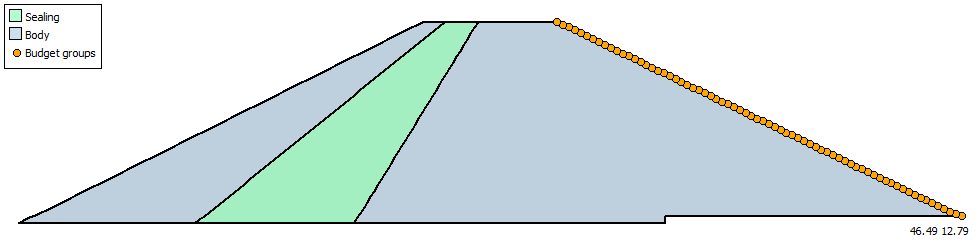
\includegraphics[width=\columnwidth]{figures/model-setup.png}
\caption{Model Setup. Water enters the dam through a Dirichlet boundary condition on the left (not shown), and flows through the sealing (green) and body areas (blue grey). The total flux of the seepage face (yellow dots) is measured. Observation point 26 relates to observation hea-25.}
\label{fig:fepest:model-setup}
\end{figure}

The example model shown in \ref{fig:fepest:model-setup} is used to illustrate the example. The underlying model is the steady-state dam seepage model used in the FEFLOW training. The steady-state unsaturated FEFLOW model calculates the seepage flux through a damn for different scenarios with changing hydraulic conductivity of the dam body.

This model converges even when choosing a very strict error criterion, and can therefore be regarded as perfectly “stable” in the FEFLOW context.

Using JACTEST, the hydraulic conductivity is changed in very small increments of 0.2 \%, in a range between 7.8 m/d and 9.5 m/d (Parameter axis). The resulting flux (m3/d) is plotted on the Observation axis of Figure \ref{fig:fepest:stabil-con-body-e1-3_100it}. 

\begin{figure}
	\center
	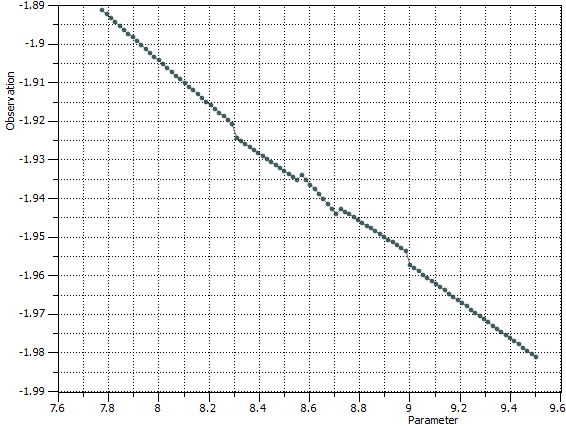
\includegraphics[width=\columnwidth]{figures/stabil-con-body-e1-3_100it.png}
\caption{Total seepage vs. hydraulic conductivity with default error criterion $1 \cdot 10^{-3}$. Discontinuities occur at various locations.}
\label{fig:fepest:stabil-con-body-e1-3_100it}
\end{figure}

The slope of the derivative is continuous along some stretches of the parameter range, however shows discontinuities of varying magnitude along the investigated parameter range. 

\subsection{Error Criterion}
The example of Figure \ref{fig:fepest:stabil-con-body-e1-3_100it} was calculated using default FEFLOW settings, with a relative error criterion of 1e-3. If reducing the error criterion by one order of magnitude (0.1 e-3 instead of 1 e-3), model granularity is strongly reduced.

\begin{figure}
	\center
	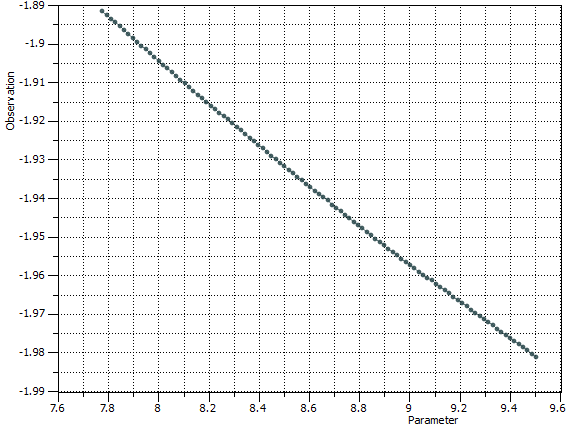
\includegraphics[width=\columnwidth]{figures/stabil-con-body-e1-4_100it.png}
\caption{Total seepage vs. hydraulic conductivity with default error criterion $1 \cdot 10^{-4}$. The reduction of the error criterion by one order of magnitude removes the discontinuities.}
\label{fig:fepest:stabil-con-body-e1-4_100it}
\end{figure}

Similar results can be found when using the L$_{max}$-error norm instead of the default RMS setting.

The non-linear iteration stops when the norm of residual head changes between two consecutive iterations falls below the termination criterion. 

This “good enough” approach allows for a degree of variability of the results - which is proportional to the magnitude of the termination criterion – must be smaller than the observation changes due to the incremental parameter change.

Therefore, FEFLOW models that are subject to a PEST optimization should have an error criterion stricter than FEFLOWs default value.

\subsection{Solver Settings}

The (linear) matrix equation solver is a second source of variability of the result. The initial example has used FEFLOWs default iterative solver PCG.

To investigate the influence of the solver error on the derivative calculation, the alternative direct solver PARDISO has been used to repeat the study. As a direct solver, PARDISO solves the matrix equations by means of analytical equations instead of iterations, and works therefore with a high accuracy independent of an error criterion.

Repeating the study with PARDISO and also the algebraic multi-grid solver SAMG 2.7, no difference between the results of simulations using the different solvers have been found.

